\usetikzlibrary{arrows.meta}
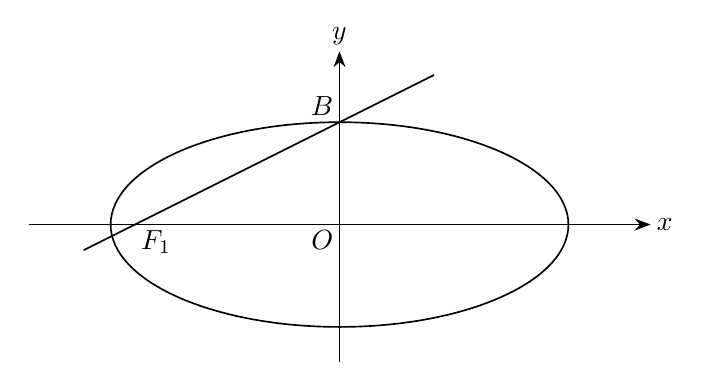
\begin{tikzpicture}[x=1cm,y=1cm,line width=.6pt,>=Stealth,font=\normalsize]
\coordinate (O) at (0,0);
\coordinate (F1) at (-2.6,0);
\coordinate (B) at (0,1.3);
\coordinate (X0) at (-3.95,0);
\coordinate (X1) at (3.95,0);
\coordinate (Y0) at (0,-1.75);
\coordinate (Y1) at (0,2.2);
\coordinate (L0) at (-3.25,-0.325);
\coordinate (L1) at (1.2,1.9);
\draw[->] (X0) -- (X1);
\draw[->] (Y0) -- (Y1);
\draw (O) ellipse[x radius=2.90689cm,y radius=1.3cm];
\draw (L0) -- (L1);
\node[anchor=north east,inner sep=0pt,xshift=-2pt,yshift=-2pt] at (O) {$O$};
\node[anchor=north west,inner sep=0pt,xshift=2pt,yshift=-2pt] at (F1) {$F_{1}$};
\node[anchor=south east,inner sep=0pt,xshift=-2pt,yshift=2pt] at (B) {$B$};
\node[anchor=west,inner sep=0pt,xshift=2pt] at (X1) {$x$};
\node[anchor=south,inner sep=0pt,yshift=2pt] at (Y1) {$y$};
\end{tikzpicture}
